\documentclass{article}
\newcommand{\classname}{CMPUT~261}
\newcommand{\termname}{Winter~2024}
\newcommand{\duedate}{Wednesday, March 27/2024}
\newcommand{\assignNum}{3}

\usepackage{enumerate}
\usepackage{booktabs}
\usepackage{amsmath, amsthm, amsfonts}
\usepackage{dsfont}
\usepackage{graphicx}
\graphicspath{{./}{qs/}}
\usepackage{color}
\usepackage[verbose,letterpaper,top=1.25in,bottom=1in,left=1.25in,right=1.25in]{geometry}
\usepackage{lastpage}
\usepackage{sgamevar}

\setlength{\parindent}{0pt}
\setlength{\parskip}{\baselineskip}

\newcounter{totalpoints}
\setcounter{totalpoints}{0}

\newcommand{\question}[2][]{(\textbf{#2}; \subtotal{#1})}
\newcommand{\subtotal}[1]{\newcounter{#1}\setcounter{#1}{0}\regtotcounter{#1}\total{#1} points}
\newcommand{\points}[2][]{{\addtocounter{totalpoints}{#2}\ifx&#1&\else\addtocounter{#1}{#2}\fi\textbf{[#2 points]}}}

\newcommand{\qsFile}[1]{}
\newcommand{\ansFile}[1]{}

\usepackage{environ}
\usepackage{etoolbox}
\makeatletter
\NewEnviron{answer}[1]
{\ifx\BODY\@empty
\vspace{#1}%
\else\ifdefined\noanswers
\vspace{#1}%
\else
{\sf\color{blue} \BODY}%
\fi\fi}
\makeatother

\usepackage{totcount}
\regtotcounter{totalpoints}
\begin{document}

{\bigskip\hrule\bigskip
\huge
\noindent \classname{}, \termname{}\\
Assignment \#\assignNum{}

\large
Due: \duedate{}\\
Total points: \total{totalpoints}

For this assignment use the following consultation model:
\begin{enumerate}

\item you can discuss assignment questions and exchange ideas with other \emph{current} \classname{} students;

\item you must list all members of the discussion in your solution;

\item you may {\bf not} share/exchange/discuss written material and/or code;

\item you must write up your solutions individually;

\item you must fully understand and be able to explain your solution in any amount of detail as requested by the instructor and/or the TAs.

\end{enumerate}

Anything that you use in your work and that is not your own creation must be properly cited by listing the original source. Failing to cite others' work is plagiarism and will be dealt with as an academic offence.


\bigskip\bigskip\hrule\bigskip

\vspace{1cm}
\hspace{1cm}{\bf First name:} \underline{\hspace{7cm}}

\vspace{1cm}
\hspace{1cm}{\bf Last name:} \underline{\hspace{7cm}}

\vspace{1cm}
\hspace{1cm}{\bf CCID:} \underline{\hspace{5.5cm}}\verb|@ualberta.ca|

\vspace{1cm}
\bigskip\hrule\bigskip
}

\pagestyle{myheadings}
\markboth{}{\classname{} --- Assignment \#\assignNum{}}

\clearpage




\begin{enumerate}





%------------------------------------------------------------------------------------------
\item \question[neural]{Neural Networks}
\label{q:code}
The MNIST dataset is a set of images of handwritten digits labelled by their actual digit.
We will operate on two versions of this dataset: one with the images shifted 2 pixels to the upper-left, and one with the images shifted 2 pixels to the bottom-right.

This question requires the use of PyTorch.  You may need to install PyTorch using the following command:
\begin{verbatim}
pip3 install --user torch torchvision
\end{verbatim}

\paragraph{Torch idiosyncrasies.}
In class, we specified the units in a dense feedforward network as performing a linear combination followed by an activation function application (e.g., relu of linear combination).  However, PyTorch treats these operations as separate layers.  See the implementation of \verb|MLP1| for an example: The hidden layer is specified as a \verb|Linear| layer followed by a \verb|ReLU| layer.  Similarly, to specify a convolutional layer with ReLU activation, you first specify a \verb|Conv2d| layer followed by a \verb|ReLU| layer.

\begin{answer}{0pt}
    % Answer here
\end{answer}

\begin{enumerate}
\item\points[neural]{10}
Implement a fully-connected feed-forward neural network for classifying MNIST images according to the digit that they represent by editing the \verb|MLP2| class in the provided \texttt{cnn.py} file.

The network should have two hidden layers: one dense linear layer with 128 rectified linear (`relu') activation, and one with  64 rectified linear units.
The output should be a fully-connected linear layer of 10 units with the softmax activation.  The \texttt{cnn.py} file contains an example implementation of a network with a single hidden layer in the \verb|MLP1| class that you may template from.  The \verb|main| function will test your program for you; you may add any tests that you like.

We will run your code by importing the \verb|cnn| module and training and evaluating the model implemented by \verb|MLP2|, so it is important that your code follow these naming conventions.

Submit all of your code for this question (including provided boilerplate files) in a single zip file.

\item\points[neural]{30}
Implement a convolutional neural network for classifying MNIST images by editing the \verb|CNN| class in the provided \texttt{cnn.py} file.

The network should have the following architecture:
\begin{itemize}
\item A layer of 32 convolutional units with a kernel size of $5\times5$ and a stride of $1,1$, with relu activation
\item A max-pooling layer with a pool size of $2\times2$ and a stride of $2,2$.
\item A layer of 64 convolutional units with a kernel size of $5\times5$ and the default stride, with relu activation.
\item A max-pooling layer with a pool size of $2\times2$ and the default stride.
\item A \verb|Flatten| layer (to reshape the image from a 2D matrix into a single long vector)
\item A layer of 512 fully-connected linear units with relu activation
\item A layer of 10 fully-connected linear units with log-softmax activation (the output layer).
This gives an output of log-probabilities.
\end{itemize}

Submit all of your code for this question (including provided boilerplate files) in a single zip file.
\clearpage
\item \points[neural]{2} \label{q:mlp2}
What was the accuracy of your trained 2-hidden-layer feedforward network on the two test sets?
\begin{answer}{2\baselineskip}
    % Answer here
\end{answer}

\item \points[neural]{2} \label{q:cnn}
What was the accuracy of your trained convolutional neural network on the two test sets?
\begin{answer}{2\baselineskip}
    % Answer here
\end{answer}

\item \points[neural]{10}
Did one of your implementations perform substantially better on one of the test sets than the other implementation did?
If so, why?  If not, why not?
\begin{answer}{1.5in}
    % Answer here
\end{answer}


\end{enumerate}





%------------------------------------------------------------------------------------------
\item \question[bayes]{Bayesian Learning}

Suppose that you have three models ($\theta_1,\theta_2,\theta_3$) of changes in the price of a single stock.
You know that one of these models is the true model.  Each model gives the probability that tomorrow's price will be higher than today's price ($y_{t+1}$), based on whether today's price was higher than the price the day before ($y_t$).  So you can make money on average by buying the stock when $p(y_{t+1} \mid y_t, \theta^*) > .5$ and selling when $p(y_{t+1} \mid y_t, \theta^*) < .5$, where $\theta^*$ is the true model.

Your prior belief is that $\theta_1$ and $\theta_2$ are equally likely to be true, and $\theta_3$ is three times more likely than $\theta_1$ to be true.

You have a dataset $D$ of past observations, and you have computed that
\begin{align*}
p(D \mid \theta_1) &= .0210 \\
p(D \mid \theta_2) &= .0168 \\
p(D \mid \theta_3) &= .0014.
\end{align*}

\begin{enumerate}
\item \points[bayes]{6}
What are the posterior probabilities of each model being the true model?
\begin{answer}{1.5in}
    % Answer here
\end{answer}

\clearpage
\item \points[bayes]{4}
Now suppose that you run each model, and they make the following predictions:
\begin{align*}
p(y_{t+1} \mid y_t, \theta_1) &= .4 \\
p(y_{t+1} \mid y_t, \theta_2) &= .75 \\
p(y_{t+1} \mid y_t, \theta_3) &= .6.
\end{align*}

What is the maximum a posterior estimate $p(y_{t+1} \mid y_t, \hat\theta_{\text{MAP}})$?
Based on the MAP estimate, would you be better off buying or selling?

\begin{answer}{1.5in}
    % Answer here
\end{answer}

\item \points[bayes]{4}

What is the estimate according to the posterior predictive distribution for $p(y_{t+1} \mid y_t)$?
(I.e., using model averaging.)
Based on the PPD, would you be better off buying or selling?

\begin{answer}{1.5in}
    % Answer here
\end{answer}
\end{enumerate}

\clearpage



%------------------------------------------------------------------------------------------
\item \question[autodiff]{Automatic Differentiation}

Consider the following feedforward neural network:

\begin{center}
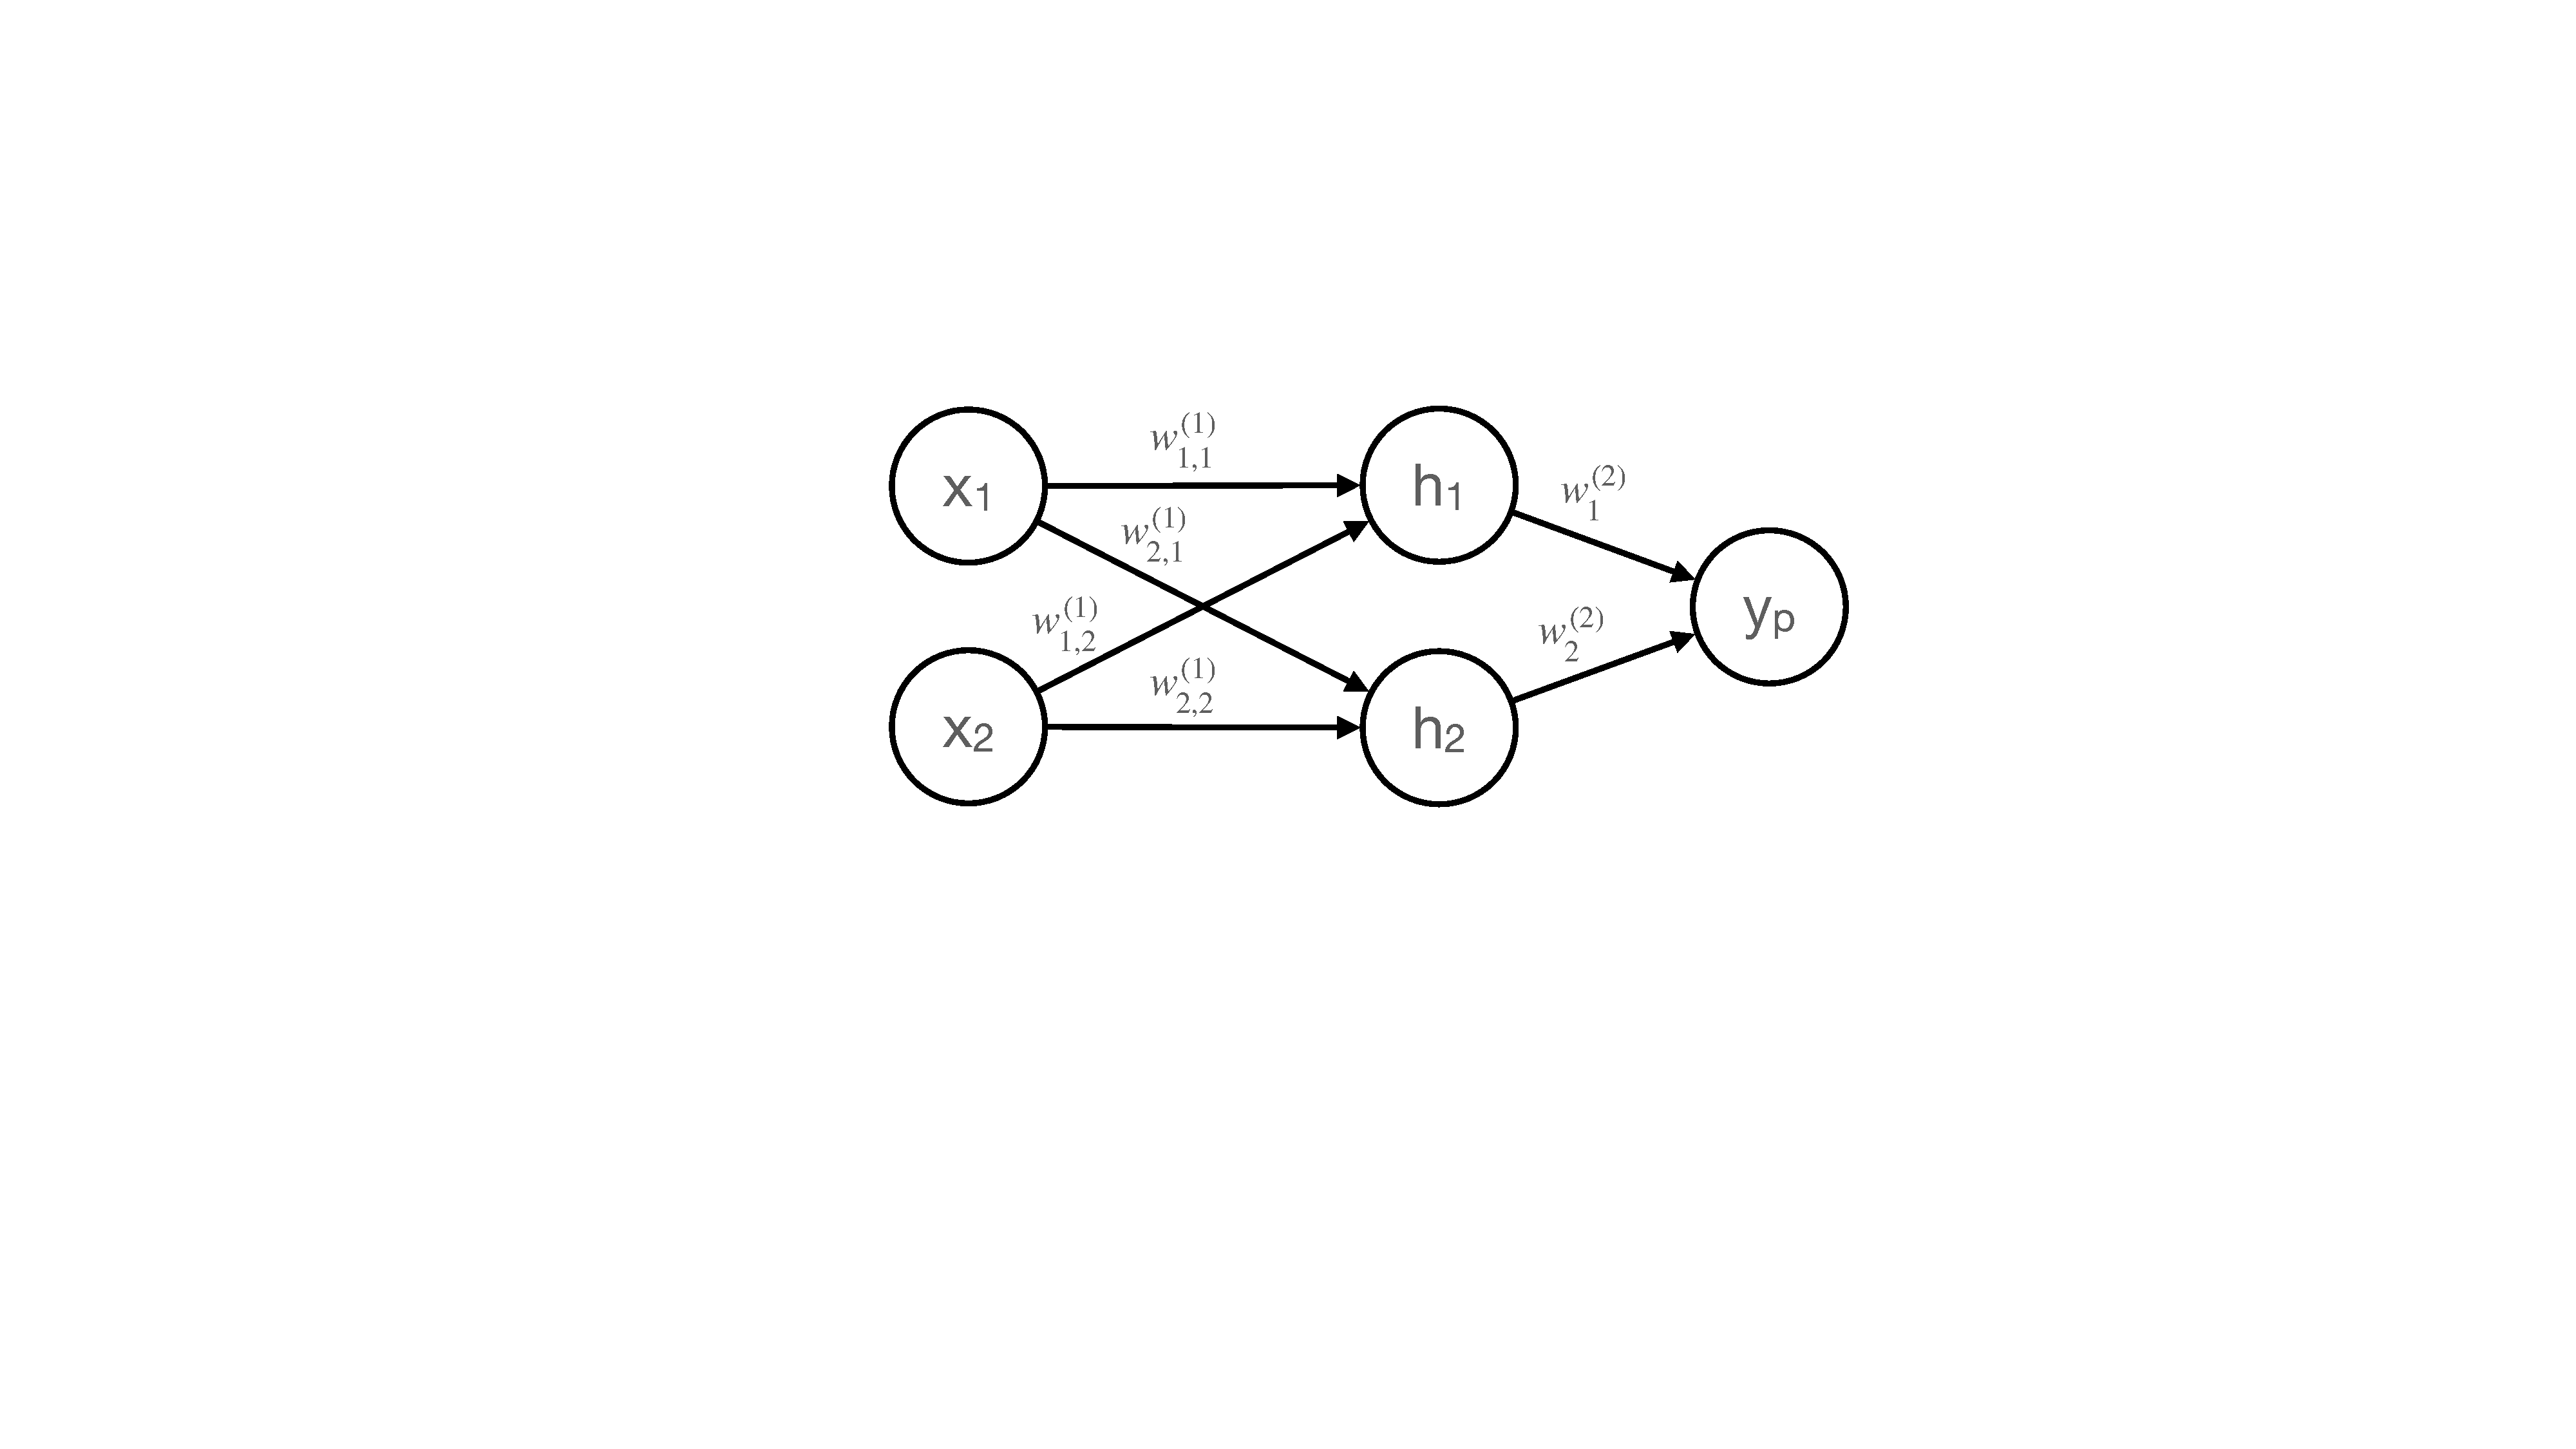
\includegraphics[width=.5\textwidth]{feedforward.pdf}
\end{center}

\begin{itemize}
\item Nodes $x_1$ and $x_2$ are input nodes.
\item Nodes $h_1,h_2,$ and $y_p$ are rectified linear units; i.e., they use the activation $g(t) = \max\{0, t\}$.
\item The inputs to $h_1$ are weighted by $w^{(1)}_{1,1}$ and $w^{(1)}_{1,2}$; $h_2$'s inputs have weights $w^{(1)}_{2,1}$ and $w^{(1)}_{2,2}$
\item The inputs to $y_p$ are weighted by $w^{(2)}_1$ and $w^{(2)}_2$.
(Note that the output node is called $y_p$ to distinguish it from the ``true'' value of $y$ in a training example)
\item There are no offsets in this network; the weights are the only parameters
\end{itemize}

\begin{enumerate}
\item \points[autodiff]{5}
Let $y_p = f\left(x_1,x_2;w^{(1)}_{1,1}, w^{(1)}_{1,2}, w^{(1)}_{2,1}, w^{(1)}_{2,2}, w^{(2)}_1, w^{(2)}_2\right)$ be the prediction of the neural network on an input $x_1,x_2$.
Give an expression for $f$.

\begin{answer}{10\baselineskip}
    % Answer here
\end{answer}

\item \points[autodiff]{3}
Let $L\left(w^{(1)}_{1,1}, w^{(1)}_{1,2}, w^{(1)}_{2,1}, w^{(1)}_{2,2}, w^{(2)}_1, w^{(2)}_1\right)$ be the mean-squared error of $f$ on a single example $(x_1,x_2,y)$.
Give an expression for $L$.
\begin{answer}{5\baselineskip}
    % Answer here
\end{answer}

\item \points[autodiff]{10} \label{q:fna-L}
Give a \emph{finite numerical algorithm} for computing $L$.

\begin{answer}{3in}
    % Answer here
\end{answer}

\item \points[autodiff]{13}
\newcommand{\loc}[1]{\overline{s_{#1}}}
\newcommand{\p}[2]{\frac{\partial s_{#1}}{\partial s_{#2}}}
\newcommand{\ind}{\mathds{1}}
Give a \emph{finite numerical algorithm} for computing the gradient of $L$ with respect to $\left(w^{(1)}_{1,1}, w^{(1)}_{1,2}, w^{(1)}_{2,1}, w^{(1)}_{2,2}, w^{(2)}_1, w^{(2)}_1\right)$.
You need not re-define the intermediate steps for the forward pass defined in (\ref{q:fna-L}).

\begin{answer}{4in}
    % Answer here
\end{answer}
\end{enumerate}

\end{enumerate}


\clearpage

\section*{Submission}
The assignment you downloaded from eClass is a single ZIP archive which includes this document as a PDF {\em and} its \LaTeX{} source as well as a Python file needed for Question~\ref{q:code}.
You are to unzip the archive into an empty directory, work on the problems and then zip the directory into a new single ZIP archive for submission.

\medskip

Each assignment is to be submitted electronically via eClass by the due date.
\textbf{Your submission must be a single ZIP file containing}:
\begin{enumerate}
\item a single PDF file with your answers;
\item file(s) with your Python code.
\end{enumerate}

To generate the PDF file with your answers you can do any of the following:

\begin{itemize}
\item
insert your answers into the provided \LaTeX{} source file between \verb|\begin{answer}| and \verb|\end{answer}|. Then run the source through \LaTeX{} to produce a PDF file;

\item print out the provided PDF file and legibly write your answers in the blank spaces under each question. Make sure you write as legibly as possible for we cannot give you any points if we cannot read your hand-writing. Then scan the pages and include the scan in your ZIP submission to be uploaded on eClass;

\item use your favourite text processor and type up your answers there. Make sure you number your answers in the same way as the questions are numbered in this assignment.
\end{itemize}

\end{document}
